\section{I/O Bursting Buffer Overview}
% Why I/O server in client nodes
\label{sec:burst_buffer}

%\begin

An overview of I/O burst buffer architecture and two kinds of buffer model: one-side buffer and two-side buffer are described in this section.
As we mentioned in the previous section, our model takes advantage of high throughput inside a system, and use buffer queue system in order to increase throughput between two systems.
Two kinds of buffer are used in our I/O burst buffer architecture, the first one is in client computing node, first buffer user I/O in the same node, another one is in I/O buffer nodes.
The main idea is that some of computing nodes serve as a I/O buffer nodes in each system, for write I/O data, if buffer queue in I/O buffer nodes is not full, data can first be buffered in buffer queue in the same system, and then be transferred to final storage system, and for reading, if that file is stored in the buffer queue, computing nodes can read from I/O nodes through Ethernet.
In other cases (buffer queue is full when issue a write requst or requsted file is not stored in buffer queue when issue a read request we call it cache miss), an read from or write back operation described below will be executed. 
\kento{how about read ?}.
%the same computing nodes and then these I/O buffer nodes, after that data will be  transferred to storage in another system.
%Although our goal here is to federate supercomputer with public cloud, since there are a great performance gap between normal supercomputer nodes and public cloud nodes and problem described above, here we consider about federating virtual machine nodes which running on supercomputer physical nodes with public cloud.
%Since public clouds also run virtual machine on physical nodes, in the follow section, we treat the set of supercomputer's virtual machines as a cloud environment, also because only a few public IP address available in each cloud, I/O buffer nodes are required even in direct connection model.


%Reading operation describes operations when issues reading data from another cloud storage, and writing operation describes operation when issues writing data to another cloud storage

%Migration operation occurs when some nodes have to be shut down in one cloud 
%all jobs running on these nodes have to be backed up by using snapshot, 

\subsection{Assumptions}
First, we make several assumptions for the federated environments as follows.
%For security consideration and the fact that IPv4 addresses becomes rare,
\begin{itemize}
	\item All computing nodes are connected by large bandwidth and interconnection network, note network topology maybe different in each system, so topology is not specified here, interconnection network performance is measured by throughput.
	\item There is a shared storage for date sharing inside system, all computing nodes are connected with shared storage, also the filesystem of shared storage is not specified and performance is measured by throughput.
	\item All nodes used by the same job are allocated in the same system, since the Internet bandwidth is low and unstable, user do not want to make communication between nodes via Internet.% so data consistency can be guaranteed since that.
\end{itemize}

\subsection{I/O Burst Buffer Architecture}

\begin{figure}[tb]
	\centering
	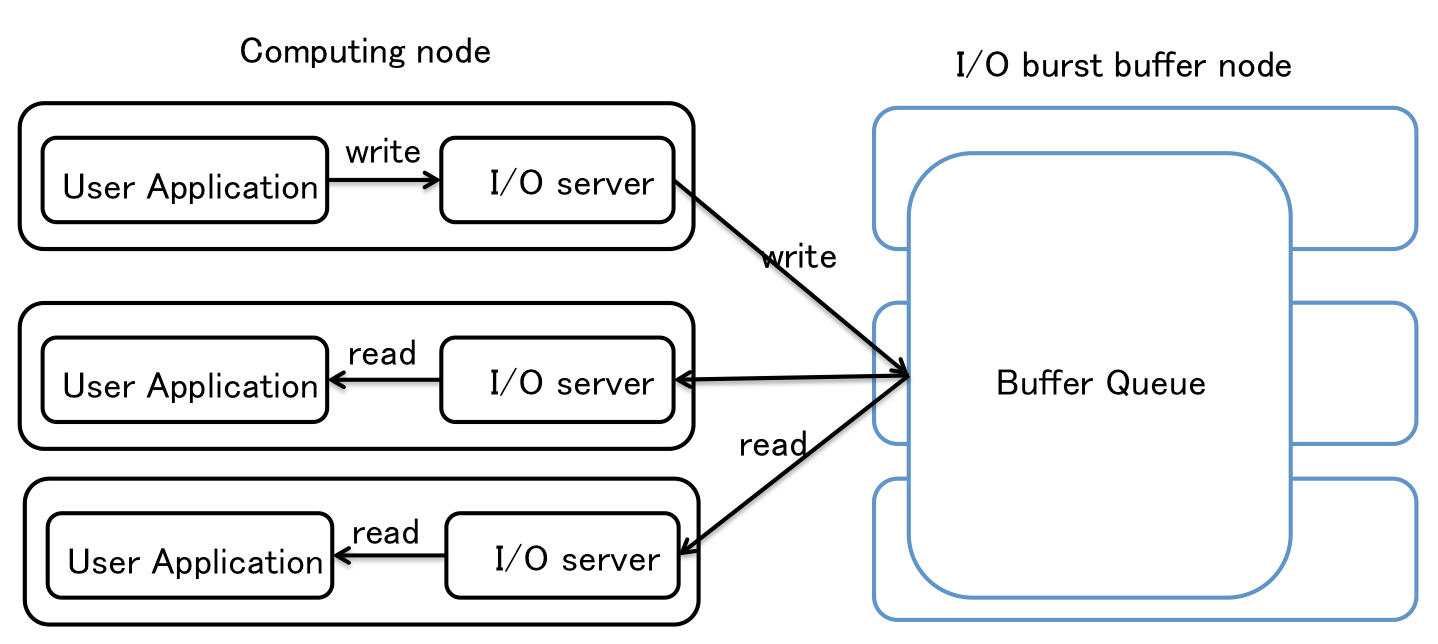
\includegraphics[width=6cm]{../img/IOserver}
	\caption{I/O server and buffer queue}
	\label{I/O server}
\end{figure}

\begin{figure}[tb]
	\centering
	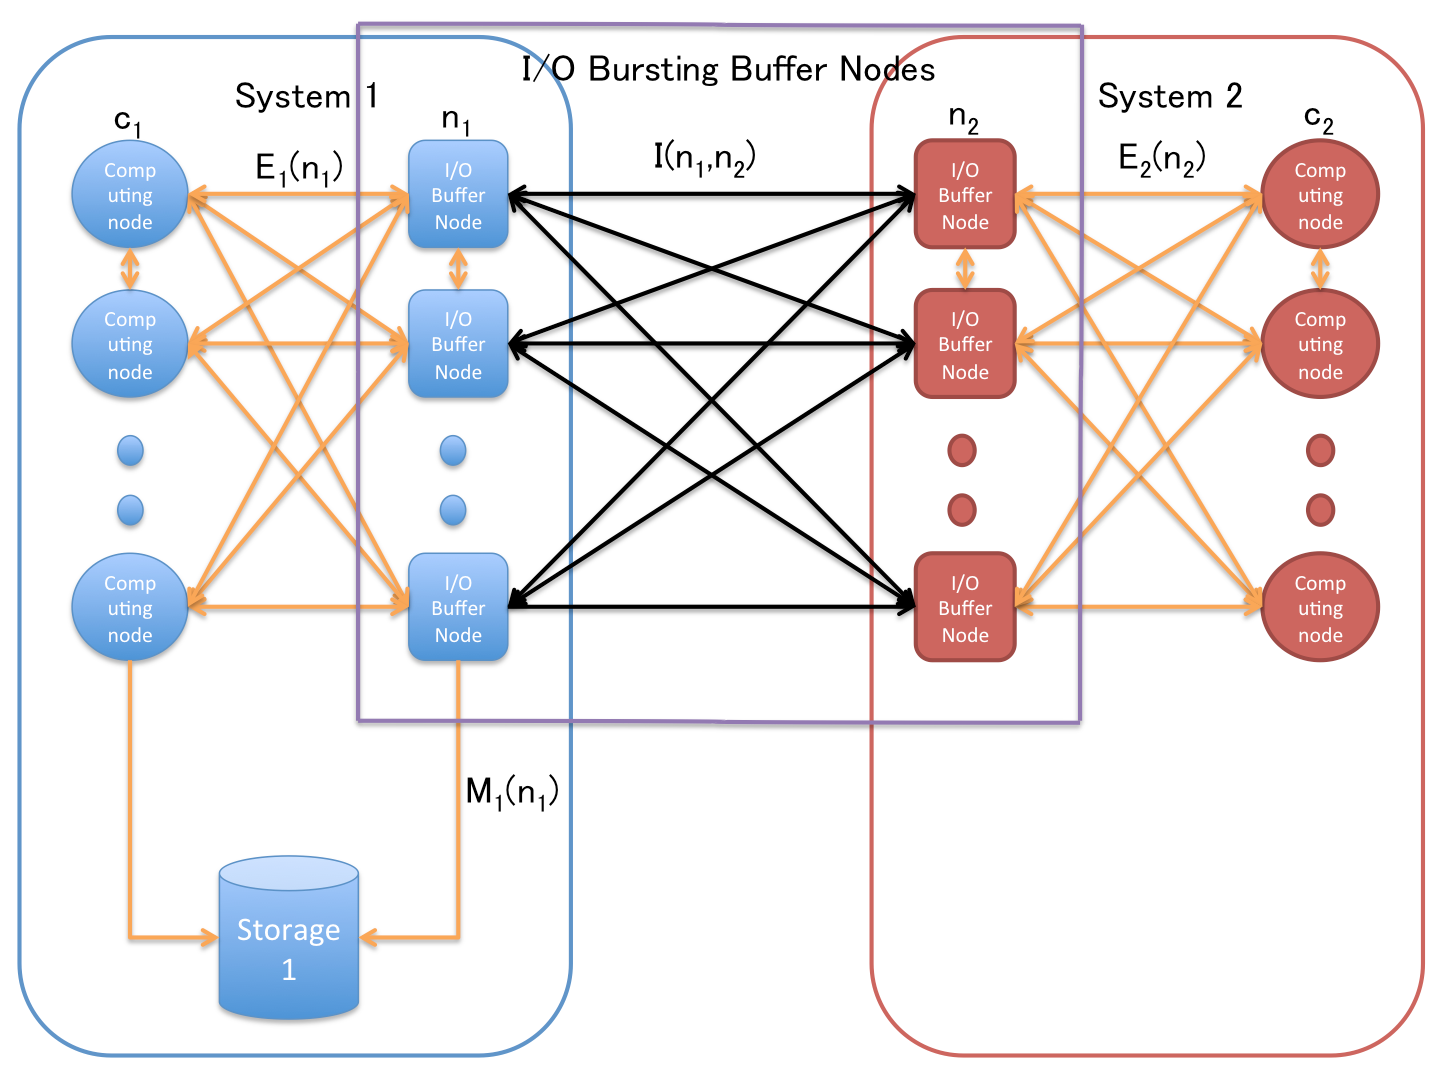
\includegraphics[width=6cm]{../img/overview}
	\caption{overall illustrate of I/O Burst Buffer Architecture}
	\label{overview}
\end{figure}

%Fig.~\ref{overview} and Fig.~\ref{I/O server} are the overall illustrate of I/O Bursting Buffer:
There are two kinds of nodes in our I/O burst buffer architecture: \emph{computing nodes} and \emph{I/O burst buffer nodes}, computing nodes run user's application and I/O burst buffer nodes.
Among I/O burst buffer nodes, there is a master nodes, which maintain a global buffer queue and a namespace, controll buffer read and write, and manage I/O buffer nodes, buffer data is distributed to all I/O buffer nodes in order to enable concurrent read and write.

Fig.~\ref{I/O server} is a illustrate of I/O server inside client nodes and buffer queue in I/O burst buffer nodes.
In each computing node, there is a I/O server, which is a filesystem client used to buffer I/O data, communicate with I/O buffer nodes, including send I/O requset and send or receive I/O data.

When a user application issue a write request, I/O data will be buffered in that node by I/O server, when user close the file, call flush function or I/O data size exceed I/O server buffer size, I/O server will try to transfer I/O data to buffer queue in I/O burst buffer, if buffer queue in not full, I/O data will be sent to I/O burst buffer via Ethernet and can be seen among computing nodes in the same system after that.
However if buffer queue is full, I/O server will block user application and wait until buffer queue is ready to recieve new I/O data, causing a low I/O throughput.

%When I/O server is notified that buffer queue is ready,first, I/O server sends the size of I/O data to master I/O burst buffer node, master node return a list of several I/O buffer nodes, then I/O server split I/O data into pieces, and sends each pieces to a I/O buffer node, after data transfer finished, that file will be added to buffer queue and namespace, and this file can be seen by all computing nodes, since we assume that all nodes used by the same job are allocated in the same system, so data consistency can be guaranteed since that.
%Buffer queue operation including data write back and operation when queue is full will be described in following section.

Similiarly when user issue a read request, there are two conditions: required file is buffered in buffer queue in I/O burst buffer, or file is stored only in storage in another system.
In the first cases, file can be transferred to computing nodes from buffer queue directly, and can achieve a high throughput.
If data is not in buffer queue, then a read operation described below will be executed, since data must be transferred from storage in another system, in this case, throughput will depend on Internet condition and it is hard to achieve a high throughput.

Fig.~\ref{overview} shows a overall illustrate of I/O burst buffer architecture.

%Consider there are two systems, named system 1 and system 2


%Arrows stand for network connection.
%Orange arrows are interconnection networks inside cloud, although two clouds used the same color for interconnection networks, bandwidth can be different, also the topolopies are not specified and can be different in each cloud.
%Black arrows are Internet connections, since there are a few amount of public IP addresses available, only I/O buffer nodes are connect to Internet, also the amount of available public IP address becomes the upper bound of the amount of I/O buffer nodes in each cloud. 
%Although nodes with private IP address can use route or other net device to connect to Internet, but consider about security problem, also using route will reduce concurrent data transfer rate, here we assume all nodes in cloud only connect to local private network except I/O buffer nodes which connect to both local network and Internet.

%Circles stand for computing nodes, which are used for standard computation.
%Here we assume all computing nodes can communicate with each other, and also I/O buffer nodes and shared storage in the same cloud environment.
%Squares are I/O buffer nodes, these nodes are used for data transfer between clouds, and are assigned with both public and private IP addresses.
%I/O buffer nodes can use the same machine or VM as computing nodes, or can use network optimized nodes for larger throughput, but it is not required here.
%Cylinders are shared storages, which are used to store data used by computing nodes, usually shared storage is consist of several nodes with a distributed filesystem and uses a better network, offers a large throughput.

%Since there is a big gap between cloud inside data transferring and accross two clouds in throughput, our goal is to fill the gap. 

%For convenience, in the following section we assume data is stored in Cloud 1's shared storage, and computing nodes in Cloud 2 are used for computation. 

%in this subsection, we introduce operations of buffer queue write back.

\subsection{Read and Write}

\begin{figure}[tb]
	\centering
	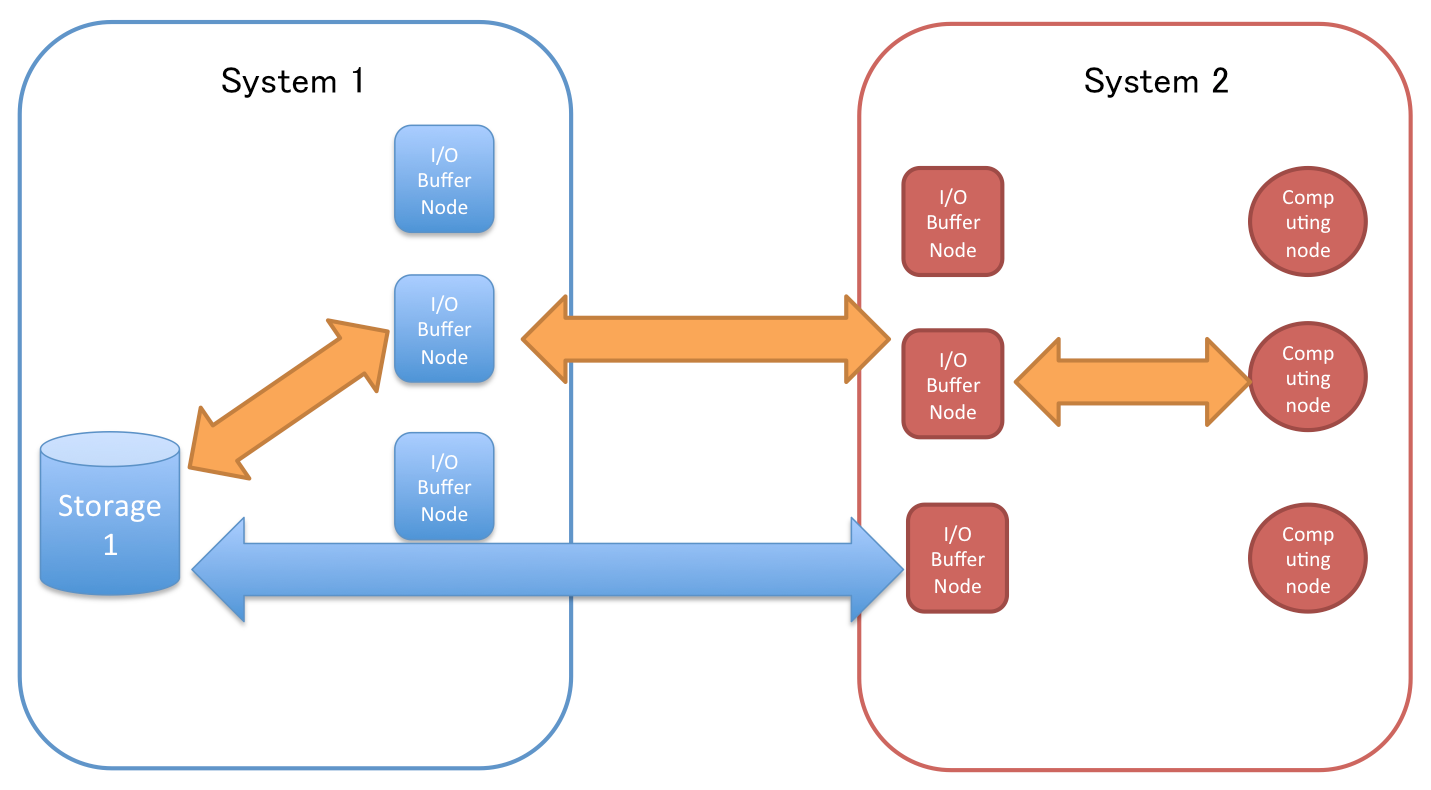
\includegraphics[width=6cm]{../img/read_and_write}
	\caption{read and write operation}
	\label{read and write}
\end{figure}

In this section we describe read and write operations when cache miss happens.%file is not in I/O buffer nodes or file needs to be write back to storage in another system.
We propose two kinds of model: one-side buffer and two-side buffer.

\subsubsection{One-side Buffer}

As Fig.~\ref{read and write} blue arrow shows, one-side buffer is a connection between I/O buffer nodes in system 2 and storage in system 1 directly.
When I/O nodes need to write data back to storage in another system, since data is already spread among I/O nodes, a parallel write can be used to fully utilize the Internet bandwidth.

Similarly, when I/O nodes need to read data from storage in another system, several I/O nodes will be assigned equal size of data, and then these nodes read assigned piece of data from the storage concurrently.

There will be two problems in this solution:
\begin{itemize}
	\item First storage should be opened to Internet, in order that I/O nodes can read from or write to it.
		However storage system in supercomputer store Petabyte of research data, open the access of storage system means that put these research data under risk of attack.
	\item As we mentioned before, throughput of one side communication is lower than two side communication, since we use SSH protocol based File system for security reason.
		also two side communication can achieve a higher throughput with fewer nodes, according to pay-as-you-go policy, reduce number of nodes can reduce cost.
\end{itemize}
%data firstly be splitted into number of I/O buffer nodes in cloud 2 pieces and assign one I/O buffer node one piece, then I/O buffer nodes start reading assigned data concurrently in order to fully utilize Internet bandwidth.
%After reading finished, I/O buffer nodes send data to each computing node Simultaneously, there data will be restructure by using protocol described below.

%Like reading, when computing nodes start to output data, first data will be buffered inside that nodes.
%After output finished, data will be splitted into number of I/O buffer nodes in cloud 2 pieces, and assign one I/O node one piece, then data will be sent to all I/O buffer nodes concurrently.
%When I/O buffer nodes received data, then they writing data back to storage in cloud 1.

\subsubsection{Two-side Buffer}

On the contrary, two-side buffer solution uses I/O buffer nodes in both two systems as Fig.~\ref{read and write} orange arrows show.
I/O data will be split twice, transferred throughput two sides of I/O buffer nodes and then reached the destination.

Consider I/O nodes in system 2 issue a write back operation, also, data is already spread among I/O nodes in system 2, each I/O node will find a pair among I/O nodes in system 1, then transfer their piece of data to system 1 concurrently.
After I/O node in system 1 received data, they write data back to storage in system 1.

Compared with one-side buffer, %two-side buffer required one more data transfer (I/O nodes to storage in the same system), if storage data transfer throuhput become a bottleneck, two-side buffer will cost more time than one-side buffer.
%Also, 
two-side buffer require both systems allocate I/O buffer nodes, if node usage is charge in both system, total cost may be larger than one-side buffer.

%the bottleneck is still Internet throughput, since interconnection is far faster than Internet.
However since two-side buffer does not read data from or write data to storage directly, it means we can compress data before transfer it, though it will take some time to compress and decompress data, when the Internet throughput is extremely low, compress and decompress time will be far smaller than tranferring time, and compress data can make more data buffered in buffer queue.
Also, unlike one-side buffer, two-side buffer do not require storage to be opened to Internet, only required several I/O nodes have access to Internet.

For these reasons, in the following section, we will use two-side buffer model as our read from and write back model in I/O burst buffer.
%I/O bursting buffer model may be used when throughput of direct connection between I/O buffer nodes and storage in different cloud is smaller then throughput between I/O buffer nodes, it is possible when storage is consist of few nodes, and direct connection will be 1-N connection, on the contrary, connection between I/O buffer nodes is N-N connection, has larger parallelism.

%When computing nodes issue read request, first we check whether the file has been cached in I/O buffer nodes in cloud 1, if not, File will be splitted into the same number of I/O buffer nodes in cloud 1, and each I/O buffer node will be assigned a piece of split, then all I/O buffer nodes start reading assigned piece of data from shared storage simultaneously to fully utilize the bandwidth.% I/O buffer nodes use a main index to refer to the data position in global data.

%After transferring data from shared storage finished, I/O buffer nodes in cloud 1 will connect with all I/O buffer nodes in cloud 2, then split data piece and into number of I/O buffer nodes in cloud 2,
%here a sub-index is used to refer to each piece's position, 
%then transfer these pieces to I/O buffer nodes in cloud 2 concurrently in order to fully utilize Internet bandwidth.

%When data transfer finished, I/O buffer nodes connect with all computation nodes which needs data, then transfer data to the corresponding position by using a index protocol described below, of cause all data transfer are done in parallel.

%Data writing operation doing the opposite operation as reading operation.
%When a computing node in cloud 2 issues data writing, output data will be first buffered by I/O server in that node.
%After output finished, I/O server connects with all I/O buffer nodes in the same cloud, and split output data into the number of I/O buffer nodes, then send each piece of data to each I/O buffer nodes Simultaneously.

%I/O buffer nodes then again split data into the number of I/O buffer nodes in cloud 1, like reading operation, here sub-index is used to refer to data position. and then start to transfer data concurrently. 

%Then I/O buffer nodes write data to storage in cloud 1.



\begin{comment}
\subsubsection{Index Protocol}

\begin{figure}[tb]
	\centering
%	\includegraphics
	\caption{index protocol}
	\label{index protocol}
\end{figure}

As Fig.~\ref{index protocol} shows, two indexs are used in this protocol: main index and sub-index.
There are two phases of data splitting in both reading and writing operation, 
\end{comment}
%\subsubsection{Node Migration}
%Node migration happens when some nodes have to be shut down due to some situation like power problem in summer, and still need to provide service to users.
%In these cases, nodes will be migrate by snapshot, usually snapshots of these nodes will first be stored into shared storage, then these snapshots will be transferred to another cloud, and start VM by using these snapshots.

%However, the low throughput between direct connection of nodes and storage in different environment will still be a bottleneck for quick migration.
%When using I/O buffer nodes 
